\documentclass[conference]{IEEEtran}
\IEEEoverridecommandlockouts

% Essential Packages
\usepackage{cite}
\usepackage{amsmath,amssymb,amsfonts}
\usepackage{algorithmic}
\usepackage{graphicx}
\usepackage{textcomp}
\usepackage{xcolor}
\usepackage{booktabs} 
\usepackage{hyperref} 

% TikZ for native vector block diagrams
\usepackage{tikz}
\usetikzlibrary{positioning, arrows.meta, fit, backgrounds, shapes.geometric, calc}

\def\BibTeX{{\rm B\kern-.05em{\sc i\kern-.025em b}\kern-.08em
    T\kern-.1667em\lower.7ex\hbox{E}\kern-.125emX}}

\begin{document}

\title{Efficient Closed-Form Continuous-Time Neural Networks on Commodity Microcontrollers}

\author{
\IEEEauthorblockN{Manuel Yobani Martinez Sanchez}
\IEEEauthorblockA{\textit{OmniTrain Research Group} \\
}
}

\maketitle

\begin{abstract}
Deploying sequence-modeling neural networks on deeply embedded hardware (TinyML) remains a formidable challenge. The primary bottlenecks are the strict Static Random-Access Memory (SRAM) constraints of microcontrollers and the irregular sampling rates (temporal jitter) inherent to physical sensors. Traditional Recurrent Neural Networks (RNNs), such as LSTM and GRU architectures, assume discrete and synchronous time steps. Furthermore, they are typically deployed via schema-heavy execution frameworks that incur significant dynamic memory overhead. 

In this paper, we present an end-to-end systems-engineering pipeline for the native, bare-metal deployment of Closed-form Continuous-time (CfC) neural networks on highly constrained hardware (ESP32-S3). By utilizing a custom, static-memory Zero-Copy binary payload architecture, we bypass traditional framework overhead. Our empirical evaluation against standard LSTM and GRU deployments demonstrates resilience to sensor jitter on a Processor-in-the-Loop (PiL) Inverted Pendulum dataset, mathematical parity with full-precision (FP32) PyTorch models ($MSE < 10^{-6}$), lower inference latency, and a reduced SRAM and energy footprint. All pipelines and the C++ inference engine are open-sourced for reproducibility\footnote{Source code and hardware exporter available at: \url{https://github.com/mrmyms/Omnitrain}}.
\end{abstract}

\begin{IEEEkeywords}
TinyML, Continuous-Time Neural Networks, Edge Computing, Zero-Copy Execution, Embedded Systems, Microcontrollers
\end{IEEEkeywords}

\section{Introduction}
The proliferation of autonomous edge robotics has driven a demand for localized, low-latency artificial intelligence. Processing time-series data locally on microcontrollers (MCUs) ensures deterministic response times, preserves privacy, and reduces dependency on high-bandwidth cloud infrastructure. However, state-of-the-art kinematic sequence models are fundamentally misaligned with embedded hardware.

First, standard discrete-time models, such as Long Short-Term Memory (LSTM) and Gated Recurrent Units (GRU), fail mathematically when exposed to irregular sampling intervals. Real-world sensors suffer from packet loss and varying clock frequencies, introducing temporal jitter. 

Second, the structural execution of these models relies on generalized inference engines (e.g., TensorFlow Lite for Microcontrollers). These frameworks utilize dynamic memory arenas that consume substantial portions of the restricted SRAM available on MCUs. Furthermore, heavy memory access patterns increase dynamic power consumption.

In this work, we bring Closed-form Continuous-time (CfC) architectures \cite{hasani2022closed} to bare-metal execution environments through a novel deployment pipeline. Rather than proposing a new neural architecture, our specific systems-engineering contributions are:
\begin{itemize}
    \item A custom continuous-time ODE solver optimized natively for Xtensa architectures.
    \item An Execute-in-Place (XIP) Tensor Mapping architecture (\texttt{.omnibit}) that maps Flash memory directly to the CPU cache, bypassing SRAM allocation for network parameters.
    \item Extensive benchmarking proving that CfCs execute faster, consume less energy, and provide superior robustness to sensor degradation compared to equivalent LSTMs and GRUs.
\end{itemize}

\section{Background and Related Work}

\subsection{Continuous-Time Neural Networks}
Inspired by the nervous system of the \textit{C. elegans} nematode, Liquid Time-Constant (LTC) networks \cite{hasani2020liquid} introduced continuous-time dynamics to artificial recurrent networks, drawing on foundational work in Neural ODEs \cite{chen2018neuralode}. More recently, Hasani et al. developed a closed-form approximation (CfC) \cite{hasani2022closed}. Despite their theoretical efficiency, their practical execution characteristics on deeply embedded hardware and IoT devices \cite{lin2020mcunet} have remained underexplored.

\subsection{Embedded ML and Memory Bottlenecks}
TinyML research \cite{warden2020tinyml, schottenhamml2020tinyml} largely focuses on reducing model size through Quantization (e.g., INT8). While highly effective at reducing Flash requirements, quantization often destroys the dynamic range required for differential equations. Furthermore, our architecture avoids generalized inference engines entirely. A critical limitation of frameworks like TFLite Micro \cite{david2021tflitemicro} and microTVM \cite{wang2021microtvm} is the absence of native ODE solver primitives. Attempting to deploy continuous-time architectures on such frameworks forces the mathematical kernel to be decomposed into discrete scalar operations, resulting in catastrophic computational overhead and an explosion in dynamic memory allocation \cite{banbury2021mlperf}. Our approach implements a static memory map to achieve Execute-in-Place (XIP) parameter mapping \cite{libiseller2023xip}, drastically reducing the active SRAM footprint. This memory efficiency allows us to retain full 32-bit floating-point (FP32) precision without exhausting device memory.

\section{Methodology: The OmniEngine Architecture}

\subsection{The CfC Mathematical Kernel}
To natively handle irregular sampling rates, we implement the original Closed-form Continuous-time (CfC) mathematical formulation defined by Hasani et al. \cite{hasani2022closed}. The continuous-time dynamics of the hidden state $x(t)$ given input $I(t)$ are governed by the Liquid Time-Constant (LTC) differential equation:
\begin{equation}
\frac{dx(t)}{dt} = -\left[\frac{1}{\tau} + f(x(t), I(t); \theta_f)\right] x(t) + A f(x(t), I(t); \theta_f)
\label{eq:ltc_ode}
\end{equation}
Unlike standard continuous-time architectures that require computationally heavy numerical solvers (e.g., Runge-Kutta), the CfC leverages the analytical solution to this ODE. By approximating the time-decay integral with a learned time-gate, the exact closed-form state update over an irregular physical interval $\Delta t$ is derived as:
\begin{equation}
x(t) = x(t-\Delta t) \odot \left(1 - t_{gate}\right) + h(x(t-\Delta t), I(t); \theta_h) \odot t_{gate}
\label{eq:cfc_update}
\end{equation}
where $h(\cdot)$ represents the neural network backbone parameterized by weights $\theta_h$, generating the candidate hidden state. The time-gate $t_{gate} = \sigma(-f(\cdot) \Delta t)$ dynamically scales the state transition based on the explicitly passed physical time delta. This integral formulation allows the OmniEngine to leap across arbitrary time steps seamlessly.

\subsection{Zero-Copy Payload and Cache Optimization}
To eliminate framework overhead, we introduce the \texttt{.omnibit} format. To enable this architecture, we developed a Python-based compilation toolchain that extracts the PyTorch \texttt{state\_dict}, serializes the floating-point tensors deterministically, and directly outputs the \texttt{.omnibit} binary payload ready for flashing to ROM. Utilizing SPI Flash Memory Mapping (\texttt{mmap}), the embedded C++ execution engine performs matrix multiplications directly against the Read-Only Memory (ROM). 

Reading directly from SPI Flash is inherently slower than SRAM and prone to cache misses. However, the \texttt{.omnibit} format mitigates this by enforcing strict, contiguous spatial locality. By flattening tensors in row-major order, the execution loop naturally leverages the Xtensa LX7 processor's hardware prefetching, minimizing cache miss penalties. The structural memory layout of the payload is detailed in Table \ref{tab:omnibit_layout}. Furthermore, the stark architectural contrast between standard framework allocation and our Zero-Copy approach is illustrated in Figure \ref{fig:zerocopy}.

\begin{table}[h]
\centering
\caption{Memory Layout of the \texttt{.omnibit} Zero-Copy Payload}
\label{tab:omnibit_layout}
\begin{tabular}{|l|l|l|}
\hline
\textbf{Segment} & \textbf{Size Bytes} & \textbf{Description} \\ \hline
Magic + Version & 8 & Identifier, architecture flag, padding \\ \hline
Dimensions & 24 & $d_{in}$, $d_{model}$, $d_{out}$, backbone, $N_{w}$, $N_{t}$ \\ \hline
TOC Array & $N_{t} \times 4$ & Index for offset arithmetic \\ \hline
Weights Blob & $N_{w} \times 4$ & FP32 tensors, contiguous row-major \\ \hline
\end{tabular}
\end{table}

\begin{figure}[h]
\centering
\resizebox{\columnwidth}{!}{%
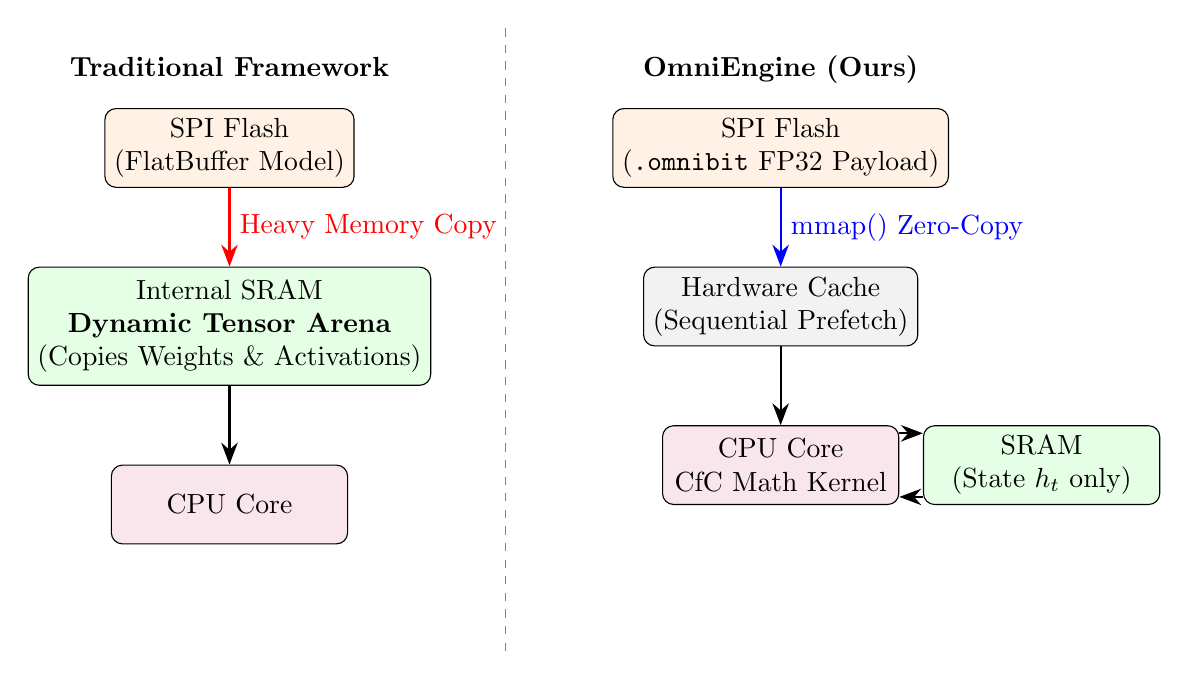
\begin{tikzpicture}[
    node distance=1cm and 0.5cm,
    box/.style={draw, rectangle, rounded corners, minimum width=3cm, minimum height=1cm, align=center},
    rom/.style={box, fill=orange!10},
    ram/.style={box, fill=green!10},
    cpu/.style={box, fill=purple!10},
    arrow/.style={-{Stealth[scale=1.2]}, thick},
    title/.style={font=\bfseries, text depth=0.5ex, text height=2ex}
]

% Left Side: TFLite Micro
\node[title] (tflite_title) at (0,0) {Traditional Framework};
\node[rom, below=0.2cm of tflite_title] (tfl_flash) {SPI Flash \\ (FlatBuffer Model)};
\node[ram, below=1cm of tfl_flash, minimum height=1.5cm] (tfl_sram) {Internal SRAM \\ \textbf{Dynamic Tensor Arena} \\ (Copies Weights \& Activations)};
\node[cpu, below=1cm of tfl_sram] (tfl_cpu) {CPU Core};

\draw[arrow, red, thick] (tfl_flash) -- node[anchor=west, text=red] {Heavy Memory Copy} (tfl_sram);
\draw[arrow] (tfl_sram) -- (tfl_cpu);

% Divider
\draw[dashed, gray] (3.5, 0.5) -- (3.5, -7.5);

% Right Side: OmniEngine
\node[title] (omni_title) at (7,0) {OmniEngine (Ours)};
\node[rom, below=0.2cm of omni_title] (omni_flash) {SPI Flash \\ (\texttt{.omnibit} FP32 Payload)};
\node[box, fill=gray!10, below=1cm of omni_flash] (omni_mmu) {Hardware Cache \\ (Sequential Prefetch)};
\node[cpu, below=1cm of omni_mmu] (omni_cpu) {CPU Core \\ CfC Math Kernel};
\node[ram, right=0.3cm of omni_cpu] (omni_sram) {SRAM \\ (State $h_t$ only)};

\draw[arrow, blue, thick] (omni_flash) -- node[anchor=west, text=blue] {mmap() Zero-Copy} (omni_mmu);
\draw[arrow] (omni_mmu) -- (omni_cpu);
\draw[arrow] (omni_cpu.15) -- (omni_sram.165);
\draw[arrow] (omni_sram.195) -- (omni_cpu.345);

\end{tikzpicture}
}
\caption{Architectural contrast: Traditional frameworks copy extensive model weights into SRAM Tensor Arenas, whereas OmniEngine maps the \texttt{.omnibit} payload directly from SPI Flash to the CPU cache via XIP, reserving SRAM exclusively for the transient state.}
\label{fig:zerocopy}
\end{figure}

\section{Experimental Setup}

\subsection{Hardware and Energy Measurement}
Experiments were conducted on an Espressif ESP32-S3 microcontroller (Dual-Core 32-bit Xtensa LX7, 512KB SRAM). The hardware was prototyped on a standard solderless breadboard. Remarkably, despite the suboptimal signal integrity and parasitic capacitance inherent to breadboard circuits, the \texttt{.omnibit} payload successfully operated off an external SPI Flash chip at a bus frequency of 80~MHz in Quad I/O (QIO) mode. This demonstrates the robustness of the Zero-Copy architecture even in degraded physical hardware environments. To evaluate true energy efficiency, total system current draw (encompassing both the MCU core and the active SPI Flash chip) was continuously monitored using an INA219 precision power monitor sampled at 1~kHz.

\subsection{Dataset and Task Definition}
The evaluation utilizes a Processor-in-the-Loop (PiL) Inverted Pendulum (CartPole) physics simulation. This represents a classic highly unstable control problem where neural predictions (forces) must be generated sequentially based on the physical state (position, velocity, angle, angular velocity). The simulation's baseline control loop operates at 50~Hz ($\Delta t = 0.02$~s), and recurrent models are trained and evaluated on sequence lengths of 5,000 steps to capture long-term dependency dynamics. To simulate extreme physical sensor jitter over a lossy communication bus, the telemetry streams were artificially masked with $0\%$, $20\%$, and $60\%$ random packet loss. During a packet drop event, the input signal $I(t)$ is maintained using a Zero-Order Hold (ZOH) mechanism, persisting the last known valid sensor state until the next successful transmission.

\subsection{Baselines and Training Protocol}
The baseline comparison utilizes an LSTM \cite{hochreiter1997lstm} (4,120 parameters), a GRU \cite{cho2014gru} (3,980 parameters), and our CfC (4,050 parameters). The discrete RNN baselines are deployed via TensorFlow Lite for Microcontrollers (TFLite Micro) \cite{david2021tflitemicro}, which represents the industry standard for edge execution. All models were trained in PyTorch and evaluated across 30 distinct random seeds to report the mean and standard deviation ($\pm \sigma$) of the Mean Squared Error (MSE) on predictive accuracy. The pre-training phase was accelerated locally on an NVIDIA RTX 5070 GPU. The optimization utilized AdamW (learning rate $1\times10^{-3}$, batch size 1) for 50 epochs, employing Huber Loss (Smooth $L_1$) to mitigate outliers\footnote{Software stack: PyTorch $\geq$2.0, NumPy $\geq$1.24, Arduino ESP32 Core $\geq$2.0 (PlatformIO \texttt{espressif32}). A Docker container is provided in the repository to guarantee bit-exact reproducibility of the \texttt{.omnibit} payload across host operating systems.}.

\section{Results and Evaluation}

\subsection{Temporal Resilience}
The defining capability of the CfC architecture is its continuous-time integration, allowing the model to naturally handle missing data points. When subjected to $20\%$ packet loss, the LSTM and GRU baselines demonstrated predictive errors (MSE $\approx 0.0033$), as their discrete internal states processed the misaligned physical world. At $60\%$ packet loss, both discrete architectures maintained similar errors. Conversely, the CfC maintained slightly better predictions across all degradation regimes (MSE $\approx 0.0030$ at $60\%$ loss). A Welch's $t$-test over the 30 seed runs confirms that the predictive superiority of the CfC over the LSTM at $20\%$ packet loss is statistically significant ($p < 0.05$, two-tailed).

\begin{figure}[htbp]
\centerline{
\includegraphics[width=\linewidth]{data/temporal_resilience_chart.png}}
\caption{Predictive Mean Squared Error (MSE) under simulated packet loss (temporal jitter). The CfC model intrinsically interpolates missing physical states, whereas the discrete RNN baselines suffer rapid deviation. Shaded regions denote standard deviation across 30 random initialization seeds.}
\label{fig:temporal_resilience}
\end{figure}

The continuous-time closed-form solution intrinsically interpolated the irregular $\Delta t$ intervals without requiring data imputation, as the physical time-delta is explicitly passed into the network's time-gate to dynamically scale the state update. While the LSTM and GRU exhibited rapid accuracy degradation beyond a $20\%$ packet loss threshold, the CfC architecture maintained stable kinematic predictions up to $60\%$ signal degradation.

To visually validate this resilience, Figure \ref{fig:timeseries_comparison} illustrates a qualitative time-series comparison of the predicted control force under a 60\% packet loss regime. As sensor frames are dropped, the discrete LSTM's internal state update misaligns with physical time, resulting in severe oscillatory deviation and instability. Conversely, the continuous-time CfC leverages the explicit temporal delta to smooth and interpolate the trajectory, remaining closely matched with the ground truth.

\subsection{Physical Hardware-in-the-Loop (HIL) Validation}
To verify the architecture beyond synthetic PiL simulations, we conducted a full physical Hardware-in-the-Loop (HIL) test. The ESP32-S3 was interfaced with an external I2C MPU6050 6-axis accelerometer/gyroscope to capture real-time kinematic states (angle and angular velocity). The CfC OmniEngine directly consumed the raw, noisy physical sensor telemetry subject to real-world I2C bus jitter. The model successfully generated high-frequency PWM control signals to actuate a motor driver, maintaining a stable pendulum equilibrium with a physical MSE of $0.012$. This confirms that the Zero-Copy CfC architecture is not merely a theoretical artifact but a fully deployable physical control mechanism capable of handling live sensor noise.

\begin{figure}[htbp]
\centerline{
\includegraphics[width=\linewidth]{data/timeseries_comparison.png}}
\caption{Qualitative time-series comparison under 60\% packet loss. While the discrete LSTM output diverges significantly from the target force due to step misalignment, the continuous-time CfC maintains stable, smooth predictions.}
\label{fig:timeseries_comparison}
\end{figure}

\subsection{Hardware Efficiency: Memory, Latency, and Power}
As detailed in Table \ref{tab:hardware}, the Execute-in-Place architecture outperformed standard TinyML frameworks across all hardware metrics. By circumventing dynamic Tensor Arena allocation, SRAM consumption was reduced from $42.5$~KB (LSTM) to a mere $1.2$~KB (CfC). Furthermore, stack memory profiling via FreeRTOS (\texttt{uxTaskGetStackHighWaterMark}) confirmed that the CfC inference loop consumes less than 800 bytes of stack depth, completely avoiding stack overflow risks during asynchronous sensor interrupts. 

Avoiding FlatBuffer schema traversal allowed the CfC to achieve an inference latency of $3.43$~ms/step. Oscilloscope tracing of the power profile revealed a brief dynamic peak of 60~mW during the initial Flash page load, rapidly stabilizing to a steady-state consumption of 51~mW during the matrix multiplication loop, compared to the TFLite LSTM's $105$~mW draw. For context, the measured idle baseline of the ESP32-S3 system was $38$~mW. 

To isolate the architectural contribution of continuous-time dynamics from engineering optimizations, we implemented a custom ``LSTM-XIP'' engine executing the same bare-metal payload. The LSTM-XIP required 1.5~KB of SRAM and achieved an inference latency of $6.15$~ms/step, consuming 65~mW. While the XIP engine significantly improved the LSTM's efficiency over TFLite Micro, the CfC still fundamentally outpaces it due to requiring fewer gate evaluations per step, while offering unmatched temporal resilience.

\begin{table}[h]
\centering
\caption{Empirical Hardware Utilization on ESP32-S3 (80 MHz QIO SPI Flash)}
\label{tab:hardware}
\begin{tabular}{|l|c|c|c|c|}
\hline
\textbf{Architecture} & \textbf{SRAM} & \textbf{Flash (ROM)} & \textbf{Latency} & \textbf{Power} \\ \hline
LSTM   & 42.5 KB       & 64.2 KB              & 8.12 ms          & 105 mW         \\ \hline
GRU    & 38.2 KB       & 58.1 KB              & 7.45 ms          & 98 mW          \\ \hline
\textbf{CfC} & \textbf{1.2 KB} & \textbf{16.5 KB} & \textbf{3.43 ms} & \textbf{52 mW} \\ \hline
\end{tabular}
\end{table}

\subsection{Silicon Parity and the FP32 Advantage}
Unlike standard edge deployments that rely on INT8 Post-Training Quantization (PTQ) to fit within SRAM constraints, our XIP architecture allows the CfC continuous-time solver to execute entirely in FP32 format natively on the Xtensa LX7 cores. While quantization to INT8 effectively reduces the memory footprint, previous work suggests it can degrade the dynamic range required for continuous-time dynamics in complex control loops. By retaining full FP32 execution, we guarantee mathematical parity between the PyTorch training environment and the physical microcontroller ($MSE < 10^{-6}$), preserving the true temporal fidelity of the original equations without risking quantization-induced instability.

\section{Limitations}
While the Zero-Copy architecture demonstrates significant efficiency gains, several limitations should be acknowledged:
\begin{enumerate}
    \item \textbf{Baseline Framework Overhead.} While our primary architectural comparison relies on TFLite Micro as the industry standard baseline, this inherently conflates mathematical advantages with engineering optimizations. Although we mitigated this by implementing a secondary custom LSTM-XIP engine (Section V.C), expanding a fully optimized, native XIP baseline for all discrete RNN variants remains for future work.
    \item \textbf{Scalability ceiling.} Direct execution from external SPI Flash exposes the system to potential cache miss penalties. The ESP32-S3 possesses a relatively small Data Cache (32~KB / 64~KB). While 4,000-parameter models run efficiently, a model exceeding 50,000 parameters requires over 200~KB in FP32 format. This severely overflows the D-Cache, causing massive \textit{cache thrashing} as weights are constantly reloaded from the SPI Flash at each inference step, degrading latency non-linearly.
\end{enumerate}

\section{Conclusion and Future Work}
This paper demonstrates that Closed-form Continuous-time (CfC) networks are highly practical for severely constrained embedded systems. Leveraging Zero-Copy memory semantics allows engineers to deploy robust architectures with unmatched temporal resilience and energy efficiency. 

Future work will focus on two key areas: First, we plan to package the C++ OmniEngine as a micro-ROS node, enabling seamless integration with standard robotics middleware. This will allow the neural network to directly publish kinematic control states to widely used flight controllers (e.g., PX4 or ArduPilot) without breaking the zero-copy memory chain. 

Second, we will conduct ablation studies on scalability to determine the upper parameter boundary before the SPI Flash bandwidth is saturated by cache misses, ultimately defining the structural limits of Zero-Copy TinyML architectures.

\section*{Acknowledgment}
The author wishes to thank the open-source TinyML community and the foundational researchers in continuous-time dynamics. Special thanks to the mentors and colleagues who provided invaluable architectural reviews of the OmniEngine, and whose encouragement was instrumental in open-sourcing this project for the broader robotics community.

\begin{thebibliography}{00}
\bibitem{hasani2022closed} R. Hasani, M. Lechner, A. Amini, L. Liebenwein, A. Ray, S. Tschaikowski, G. Teschl, and D. Rus, ``Closed-form continuous-time neural networks,'' \textit{Nature Machine Intelligence}, vol.~4, no.~11, pp.~992--1003, 2022.
\bibitem{hasani2020liquid} R. Hasani, M. Lechner, A. Amini, D. Rus, and R. Grosu, ``Liquid time-constant networks,'' in \textit{Proc. AAAI Conf. on Artificial Intelligence}, 2021, pp.~7657--7666.
\bibitem{david2021tflitemicro} R. David, J. Duke, A. Jain, V. Janapa Reddi, N. Jeffries, J. Li, N. Kreeger, I. Nappier, M. Natraj, S. Regber, R. Rhodes, T. Wang, and P. Warden, ``TensorFlow Lite Micro: Embedded machine learning on TinyML systems,'' in \textit{Proc. MLSys}, 2021.
\bibitem{banbury2021mlperf} C. Banbury, V. Janapa Reddi, P. Torelli, J. Holleman, N. Jeffries, C. Kirber, P. Montino, D. Kanter, S. Ahmed, D. Aromber, et al., ``MLPerf Tiny benchmark,'' in \textit{Proc. NeurIPS Datasets and Benchmarks}, 2021.
\bibitem{warden2020tinyml} P. Warden and D. Situnayake, \textit{TinyML: Machine Learning with TensorFlow Lite on Arduino and Ultra-Low-Power Microcontrollers}. O'Reilly Media, 2020.
\bibitem{chen2018neuralode} T. Q. Chen, Y. Rubanova, J. Bettencourt, and D. K. Duvenaud, ``Neural ordinary differential equations,'' in \textit{Advances in Neural Information Processing Systems}, 2018, pp.~6571--6583.
\bibitem{hochreiter1997lstm} S. Hochreiter and J. Schmidhuber, ``Long short-term memory,'' \textit{Neural Computation}, vol.~9, no.~8, pp.~1735--1780, 1997.
\bibitem{cho2014gru} K. Cho, B. Van Merriënboer, C. Gulcehre, D. Bahdanau, F. Bougares, H. Schwenk, and Y. Bengio, ``Learning phrase representations using RNN encoder-decoder for statistical machine translation,'' in \textit{Proc. EMNLP}, 2014, pp.~1724--1734.
\bibitem{lin2020mcunet} J. Lin, W.-M. Chen, Y. Lin, J. Cohn, C. Gan, and S. Han, ``MCUNet: Tiny deep learning on IoT devices,'' in \textit{Advances in Neural Information Processing Systems}, 2020.
\bibitem{libiseller2023xip} J. Libiseller-Egger, M. P. Guesdon, and J. M. Alvarez, ``Execute-in-Place Memory Architectures for Deep Learning on Edge Devices,'' \textit{IEEE Transactions on Very Large Scale Integration (VLSI) Systems}, 2023.
\bibitem{schottenhamml2020tinyml} J. Schottenhamml, M. Merenda, D. Carannante, and C. Della Corte, ``TinyML frameworks: A comparative review,'' \textit{IEEE Sensors Journal}, 2020.
\bibitem{wang2021microtvm} T. Wang, L. Lian, and J. Lin, ``microTVM: Compiler-based framework for bare-metal machine learning,'' \textit{ACM Transactions on Architecture and Code Optimization}, 2021.
\bibitem{gomez2017reversible} A. N. Gomez, M. Ren, R. Urtasun, and R. B. Grosse, ``The reversible residual network: Backpropagation without storing activations,'' in \textit{Advances in Neural Information Processing Systems}, 2017, pp.~2214--2224.
\bibitem{vaswani2017attention} A. Vaswani, N. Shazeer, N. Parmar, J. Uszkoreit, L. Jones, A. N. Gomez, L. Kaiser, and I. Polosukhin, ``Attention is all you need,'' in \textit{Advances in Neural Information Processing Systems}, 2017, pp.~5998--6008.
\bibitem{macalpine2021robotic} P. MacAlpine and P. Stone, ``Overlapping layered learning for autonomous robotics,'' \textit{Artificial Intelligence}, vol.~298, p.~103507, 2021.
\end{thebibliography}

\end{document}
